\chapter{Result and Discussion} % Main chapter title

\label{Chapter5} % Change X to a consecutive number; for referencing this chapter elsewhere, use \ref{ChapterX}


%----------------------------------------------------------------------------------------
%	SECTION 1
%----------------------------------------------------------------------------------------
\section{Experiment 1's Results and Discussion}
The performance of participants in identifying the three vibration cycle rates—0.2, 0.5, and 1.0—is summarized in Figure~\ref{fig:ex1_results}, which shows the overall classification accuracy across all trials. Each cycle rate had a total of 30 trials (six participants with five repetitions each). The highest classification accuracy was recorded at the 1.0 cycle rate, where participants correctly identified the vibration pattern in 26 out of 30 trials, resulting in an accuracy of 86.7\%. This suggests that higher-frequency vibration rhythms with shorter pauses are more easily perceived and classified by users, likely due to their more continuous and distinct tactile sensation.

\begin{figure}[H]\centering
	\includesvg[width=0.9\textwidth, inkscapelatex=true]{Pictures/ex1_result}
	\caption{Participants' accuracy in identifying different vibration cycle rates.}\label{fig:ex1_results}
\end{figure}


At a cycle rate of 0.5, accuracy slightly decreased to 24 out of 30 trials (80\%). The lowest accuracy was observed at a cycle rate of 0.2, with participants achieving 23 out of 30 correct identifications (76.7\%). These results indicate a trend in which participant accuracy declines as the vibration rhythm slows down, leading to a more intermittent tactile sensation. %This finding aligns with previous research in haptic perception, which has shown that higher-frequency or more intense vibrotactile cues are generally easier to detect and discriminate due to stronger stimulation of tactile receptors.

The moderate reduction in accuracy at lower cycle rates may be attributed to the diminished temporal density of tactile feedback, making it more difficult for participants to form clear perceptual distinctions, especially when the vibration intervals become more sparse. Notably, even at the lowest cycle rate, participants maintained a classification rate well above chance level (33.3\%), indicating that the PWM cycle rate modulation approach provides reliably distinguishable tactile patterns.

Overall, these findings validate the effectiveness of the proposed PWM-based feedback method in delivering perceivable differences in vibrotactile rhythms. The results demonstrate that participants can accurately classify distinct cycle rates, particularly in the higher rhythm ranges, supporting the system’s suitability for conveying virtual texture granularity through simple vibration control strategies.

%%%%%%%%%%%%%%%%%%%%%%%%%%%%%%%%%%%%%%
\section{Experiment 2's Results and Discussion}
Participants' preferences for associating vibration cycle rates with the virtual textures—brick, grass, and marble—are illustrated in Figure~\ref{fig:ex2_results}. The distribution of selections demonstrates how participants mapped specific vibration rhythms to different surface types. For the brick texture, responses were equally divided between 0.2 (low cycle rate) and 0.5 (medium cycle rate), with three participants choosing each option. This split suggests that participants found both slower and moderate rhythmic vibrations to be appropriate representations of the rough and uneven characteristics of brick surfaces. Notably, no participants selected the 1.0, indicating a shared perception that fast, continuous vibrations were not suitable for representing rough textures.

\begin{figure}[H]\centering
	\includesvg[width=0.9\textwidth, inkscapelatex=true]{Pictures/ex2_result}
	\caption{Participant-selected cycle rates corresponding to virtual surface textures}\label{fig:ex2_results}
\end{figure}

In the case of the grass texture, the responses leaned toward a cycle rate of 0.5. Four out of six participants selected the medium cycle rate, while the remaining two chose 0.2. Similar to the brick condition, no participants opted for the 1.0 cycle rate for grass. This suggests that participants generally associate slower or moderate rhythmic feedback with irregular or soft textures. The preference for the 0.5 cycle rate indicates that grass, which is visually perceived as a semi-rough but flexible material, aligns best with medium vibration rhythms. This offers a balance between perceptibility and comfort.

For the marble texture, all six participants unanimously agreed that a cycle rate of 1.0 (high cycle rate) was most effective for simulating marble texture. This strong consensus suggests that fast, smooth, and continuous vibration patterns are best suited to represent smooth, hard surfaces like polished marble. This finding aligns with established tactile perception theories, which propose that dense and uninterrupted vibrational cues effectively mimic the sensation of smooth, featureless surfaces.


%%%%%%%%%%%%%%%%%%%%%%%%%%%%%%%%%%%%%%
\section{Post-Experiment Evaluation}
Alongside performance measurements, participants filled out a 12-item post-experiment questionnaire designed to evaluate their subjective impressions of virtual hand embodiment, tactile realism, and the overall quality of the VR experience. Figure~\ref{fig:questionnaire_results} displays the summarized mean scores for all questions. This evaluation offered valuable insights into participants' perceptions of the system's effectiveness in providing immersive and tactilely enriched VR interactions.

\begin{figure}[H]\centering
	\includesvg[width=0.9\textwidth, inkscapelatex=true]{Pictures/question_result}
	\caption{Participants' accuracy in identifying different vibration cycle rates.}\label{fig:questionnaire_results}
\end{figure}

The highest agreement was observed for Q10 (“I had the sensation that I could feel the texture of objects through the virtual hand”), which reached a mean score of 5.33 out of 7, indicating strong perceived effectiveness of the vibration-based texture feedback. Similarly, Q7 (“When I touched the virtual plane, it felt as if my real hand was also being touched”) and Q6 (“The tactile sensations I perceived felt naturally aligned with the virtual hand”) received high ratings (5.00 and 4.83, respectively), supporting the conclusion that the glove effectively conveyed realistic tactile sensations during virtual interactions.

Participants reported generally positive experiences regarding immersion (Q12, mean = 4.83) and tactile attribution (Q2, mean = 4.83). This indicates that the system effectively contributed to engagement and sensory alignment within the virtual environment. There was moderate agreement on the aspects of control fidelity and perceived response accuracy, with Q4 (control of the virtual hand) scoring 4.17 and Q11 (mismatch awareness) also receiving a score of 4.17. These scores suggest that while the movement synchronization between real and virtual hands is acceptable, there is room for improvement.

However, the scores related to embodiment were lower, particularly for the following statements: Q1 (“I felt as if the virtual hands were my own”; score: 3.33), Q5 (“The virtual hand was naturally connected to my body”; score: 3.17), and Q8 (“Movements felt natural”; score: 3.17). These responses indicate a diminished sense of ownership and naturalness of movement, which aligns with the current limitations of the system regarding full-hand tracking and the responsiveness of the virtual hands.

\subsection{General Discussion}  
The results indicate a strong relationship between vibration cycle rate and the perceived realism of textures. Participants consistently linked higher cycle rates to smooth textures, while lower to medium cycle rates were associated with rough or irregular surfaces. The absence of conflicting responses—such as no participants selecting high cycle rates for materials like brick or grass—further strengthens the reliability and consistency of vibration rhythm perception. Notably, this level of differentiation was achieved without altering the vibration amplitude, demonstrating that modulation of the cycle rate alone provides clear and intuitive tactile cues that convey distinct virtual material properties. 

The simplicity of the system design, combined with effective texture differentiation, highlights the suitability of this approach for lightweight, real-time haptic feedback applications in virtual reality.

Together, the experimental performance metrics and subjective questionnaire results show that the proposed PWM-based tactile feedback method significantly improves users' ability to distinguish and realistically perceive virtual textures, thereby enhancing the overall sense of immersion in virtual environments. These findings are consistent with previous literature~\cite{10.1145/3025453.3025812,10.1007/s00542-023-05486-x}.  that emphasizes the importance of tactile granularity and frequency modulation for realistic texture rendering. Moving forward, efforts should focus on strengthening the sense of embodiment, particularly by improving hand tracking fidelity and further optimizing vibration characteristics to accommodate a broader range of virtual materials. This will help achieve a more cohesive and immersive VR experience.


% When an HMD is deployed, users struggle to understand their surroundings, identify their orientation and determine where they are in relation to other objects such as walls and users in their physical space. 
% In consideration of this, it is highly likely that users wearing HMDs collide with other users and walls. 

% To resolve this problem, the proposed method employs a strategy with a time-dependent synced-rotational gain to avoid collisions between multiple VR users sharing the same physical space. The results mentioned in the previous chapter prove that the proposed method works better than the Holm's one. This chapter describes some concerns that would affect the results. 
% \section{Motion sickness}
% From Fig.~\ref{fig:SSQ_CtoS_Of_RorationEx} to Fig.~\ref{fig:SSQ_Acc_Of_RotationEx} on rotation awareness experiments, the subjects manifested symptoms at slight and moderate levels and they could continue the experiments.
% From Fig.~\ref{fig:SSQ_ConstantOfCurvatureEx} and Fig.~\ref{fig:SSQ_AccOfCurvatureEx} on curvature distance experiments, two subjects from five subjects manifested symptoms in severe level. During the experiment on curvature distance, two of the five subjects started to have eye strain and difficulty in focusing the given task at the speed of rotation of 3.2deg/s. However, they said they could overcome motion sickness if they could take a break and then I temporarily suspended them for the extra rest time of five minutes. While they had a rest time, I recommended them to see the outside of the room such as trees and the nearby buildings. After that, their motion sickness had been reduced to a low level and they continued the task and did not experience motion sickness.

% \begin{figure}[H]\centering
% 	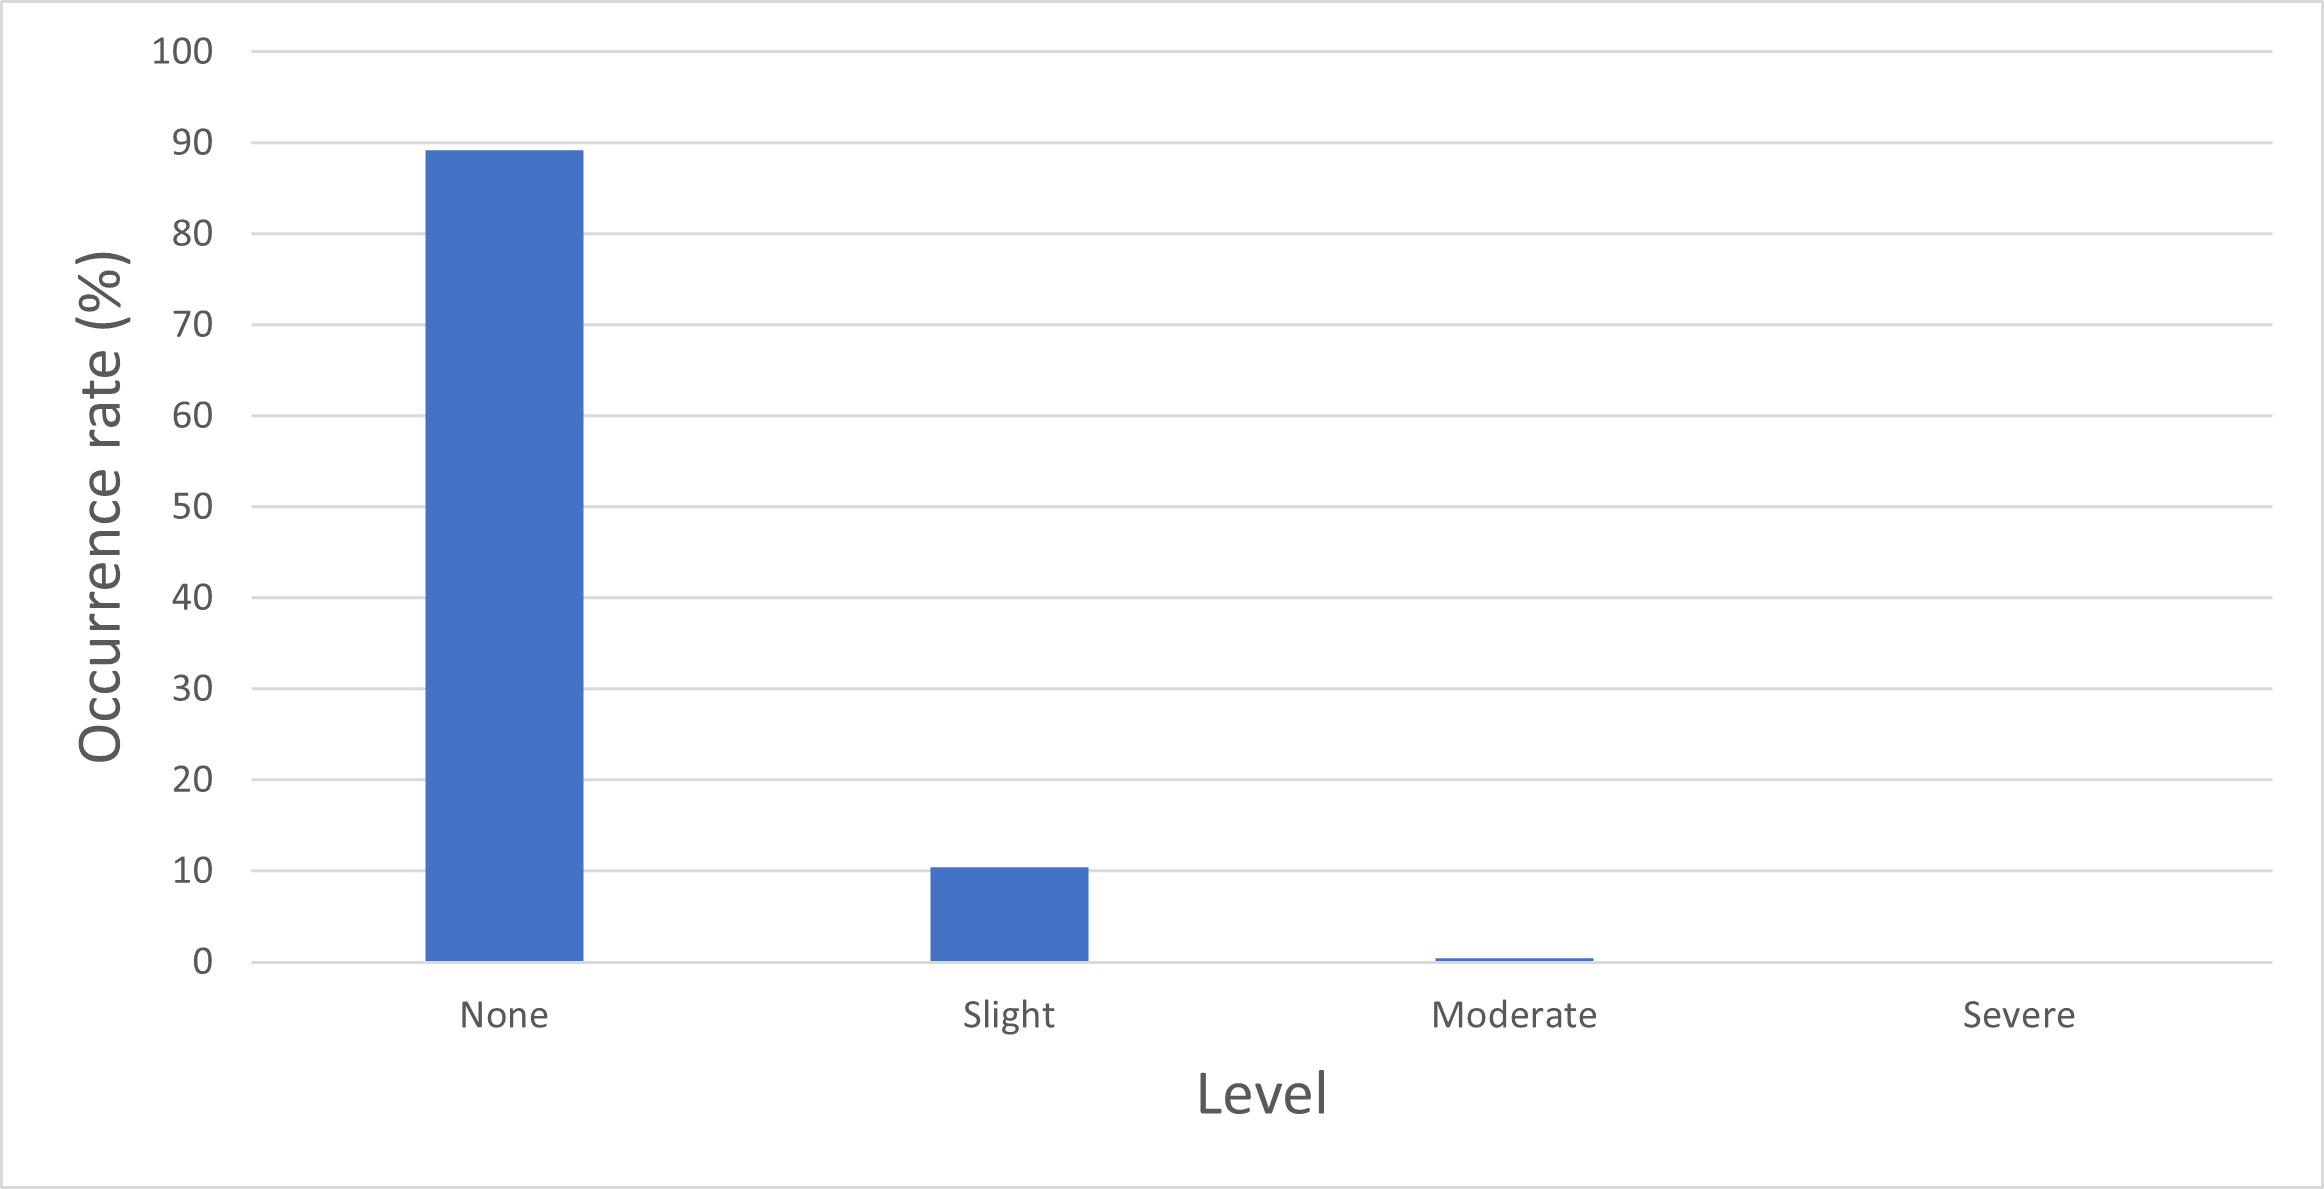
\includegraphics[width=0.9\textwidth]{Pictures/SSQ_StoC_Of_RorationEx.png}%imagine location
% 	\caption{SSQ results for the stop to constant speed rotation task.}\label{fig:SSQ_StoC_Of_RorationEx}%use name for ref.
	
% \end{figure}
% \begin{figure}[H]\centering
% 	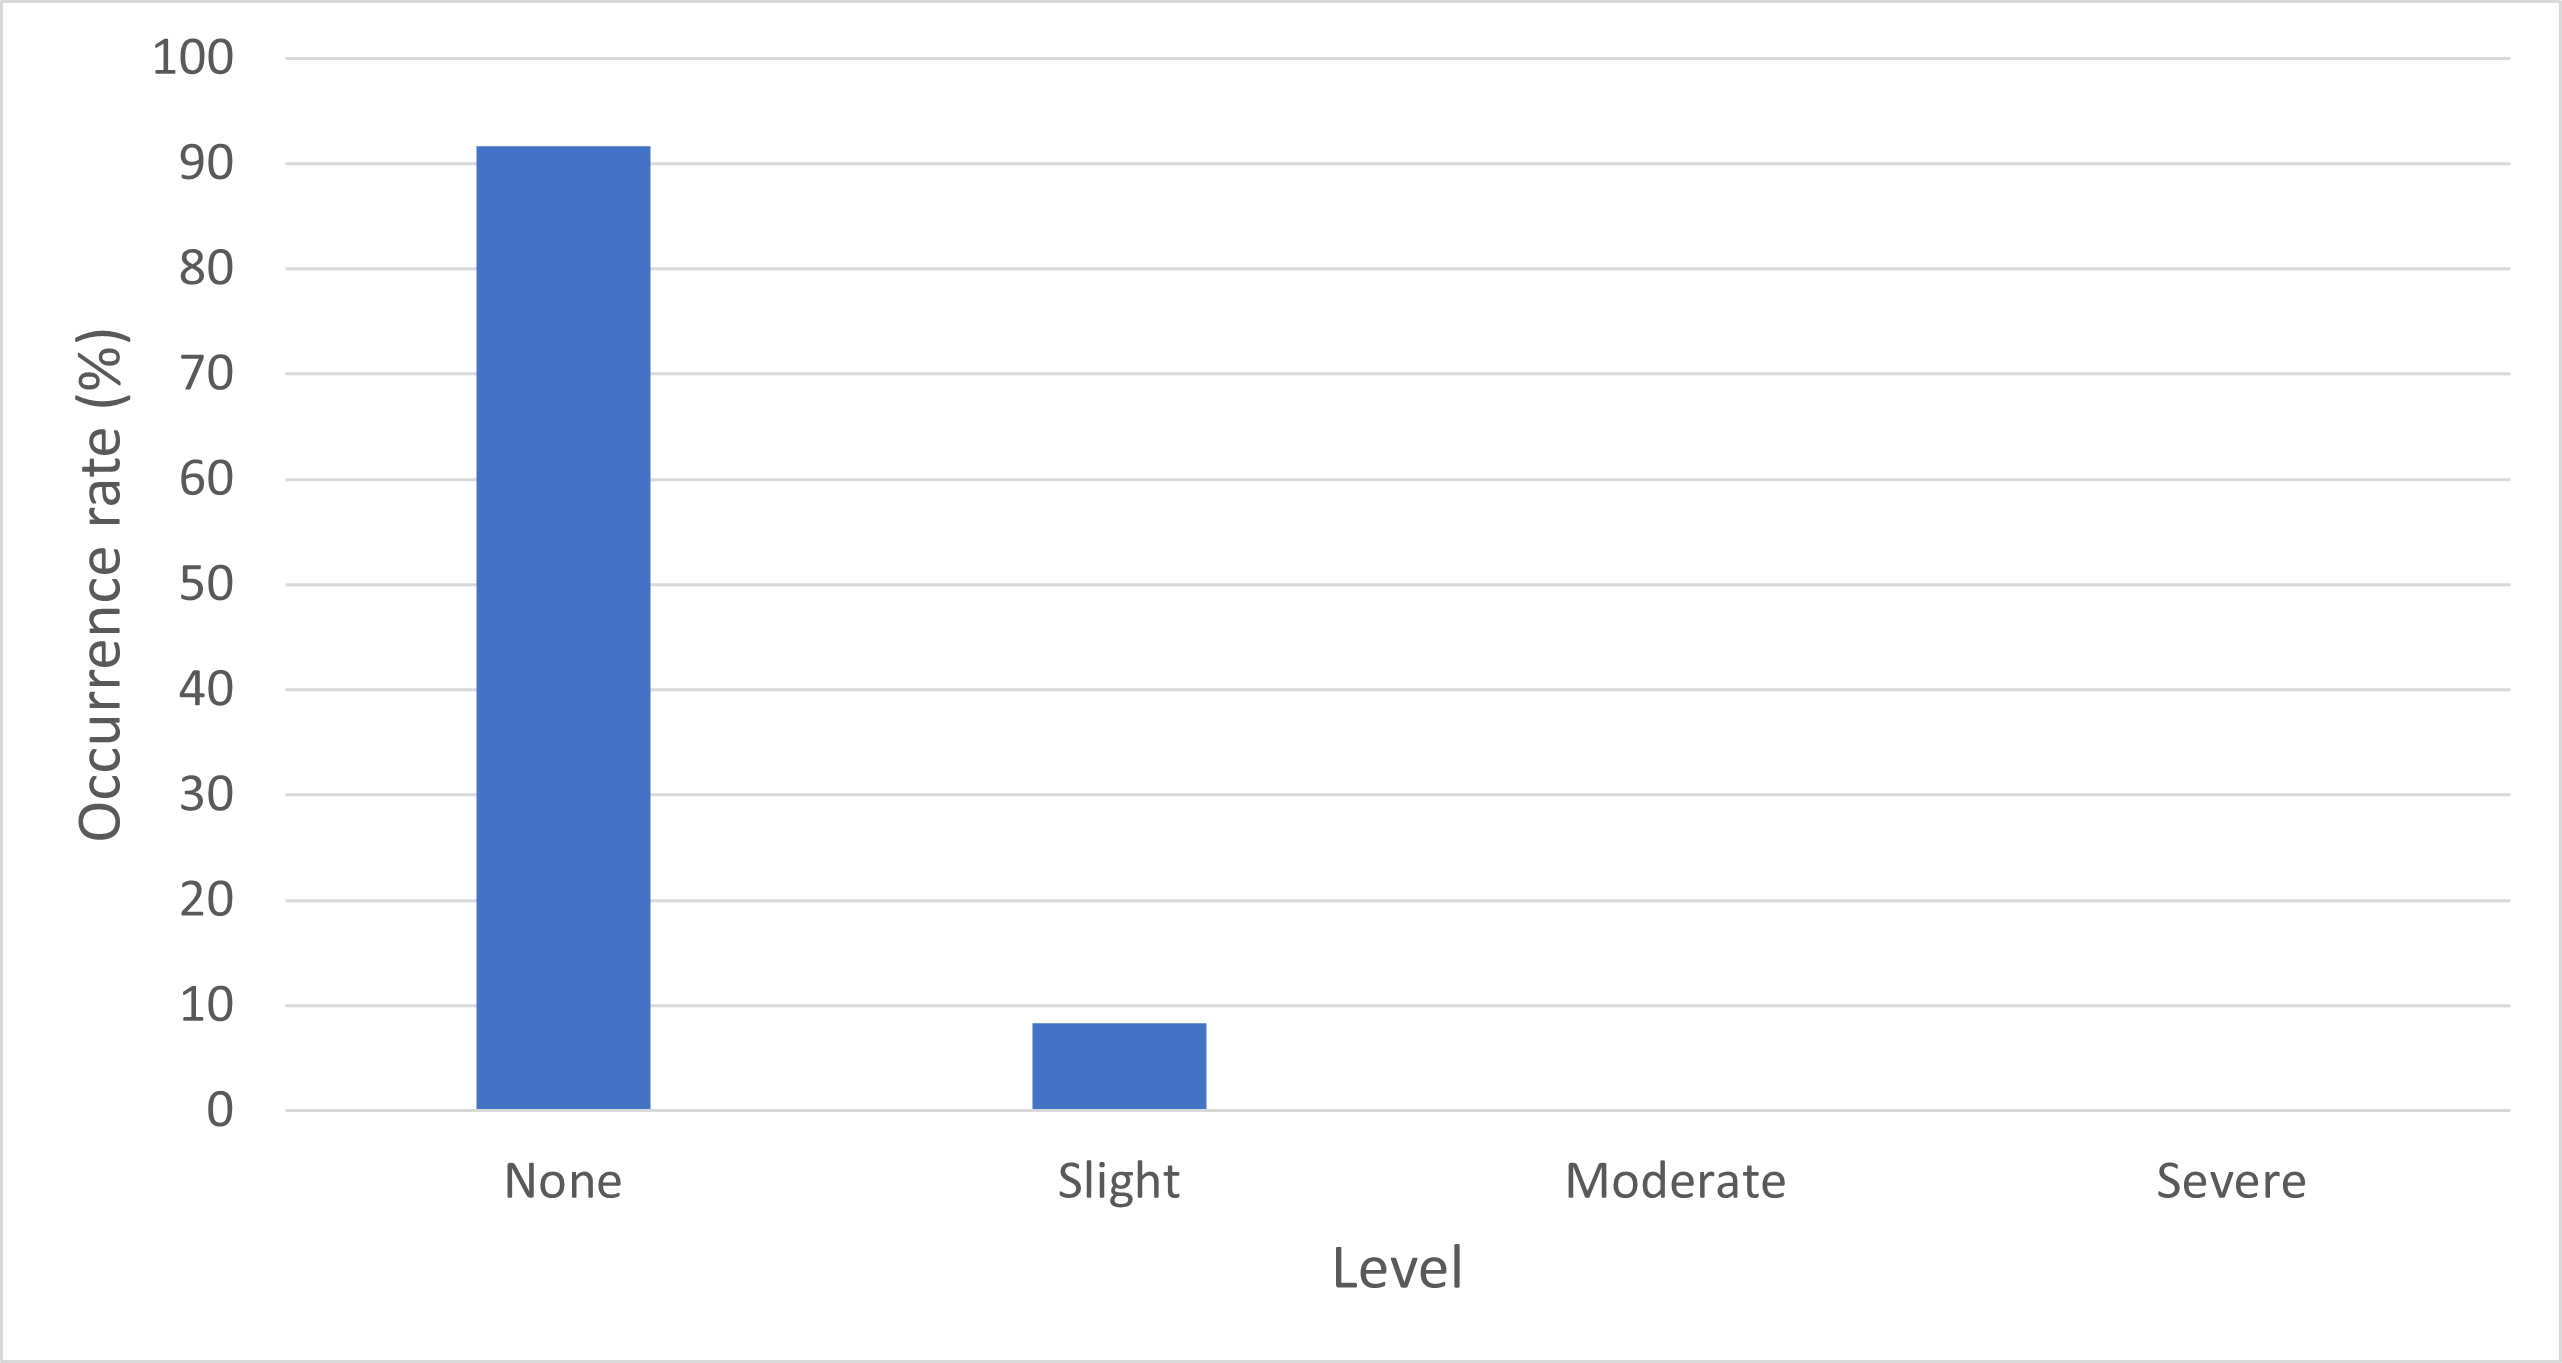
\includegraphics[width=0.9\textwidth]{Pictures/SSQ_CtoS_Of_RorationEx.png}%imagine location
% 	\caption{SSQ results for the constant speed to stop rotation task.}\label{fig:SSQ_CtoS_Of_RorationEx}%use name for ref.
	
% \end{figure}
% \begin{figure}[H]\centering
% 	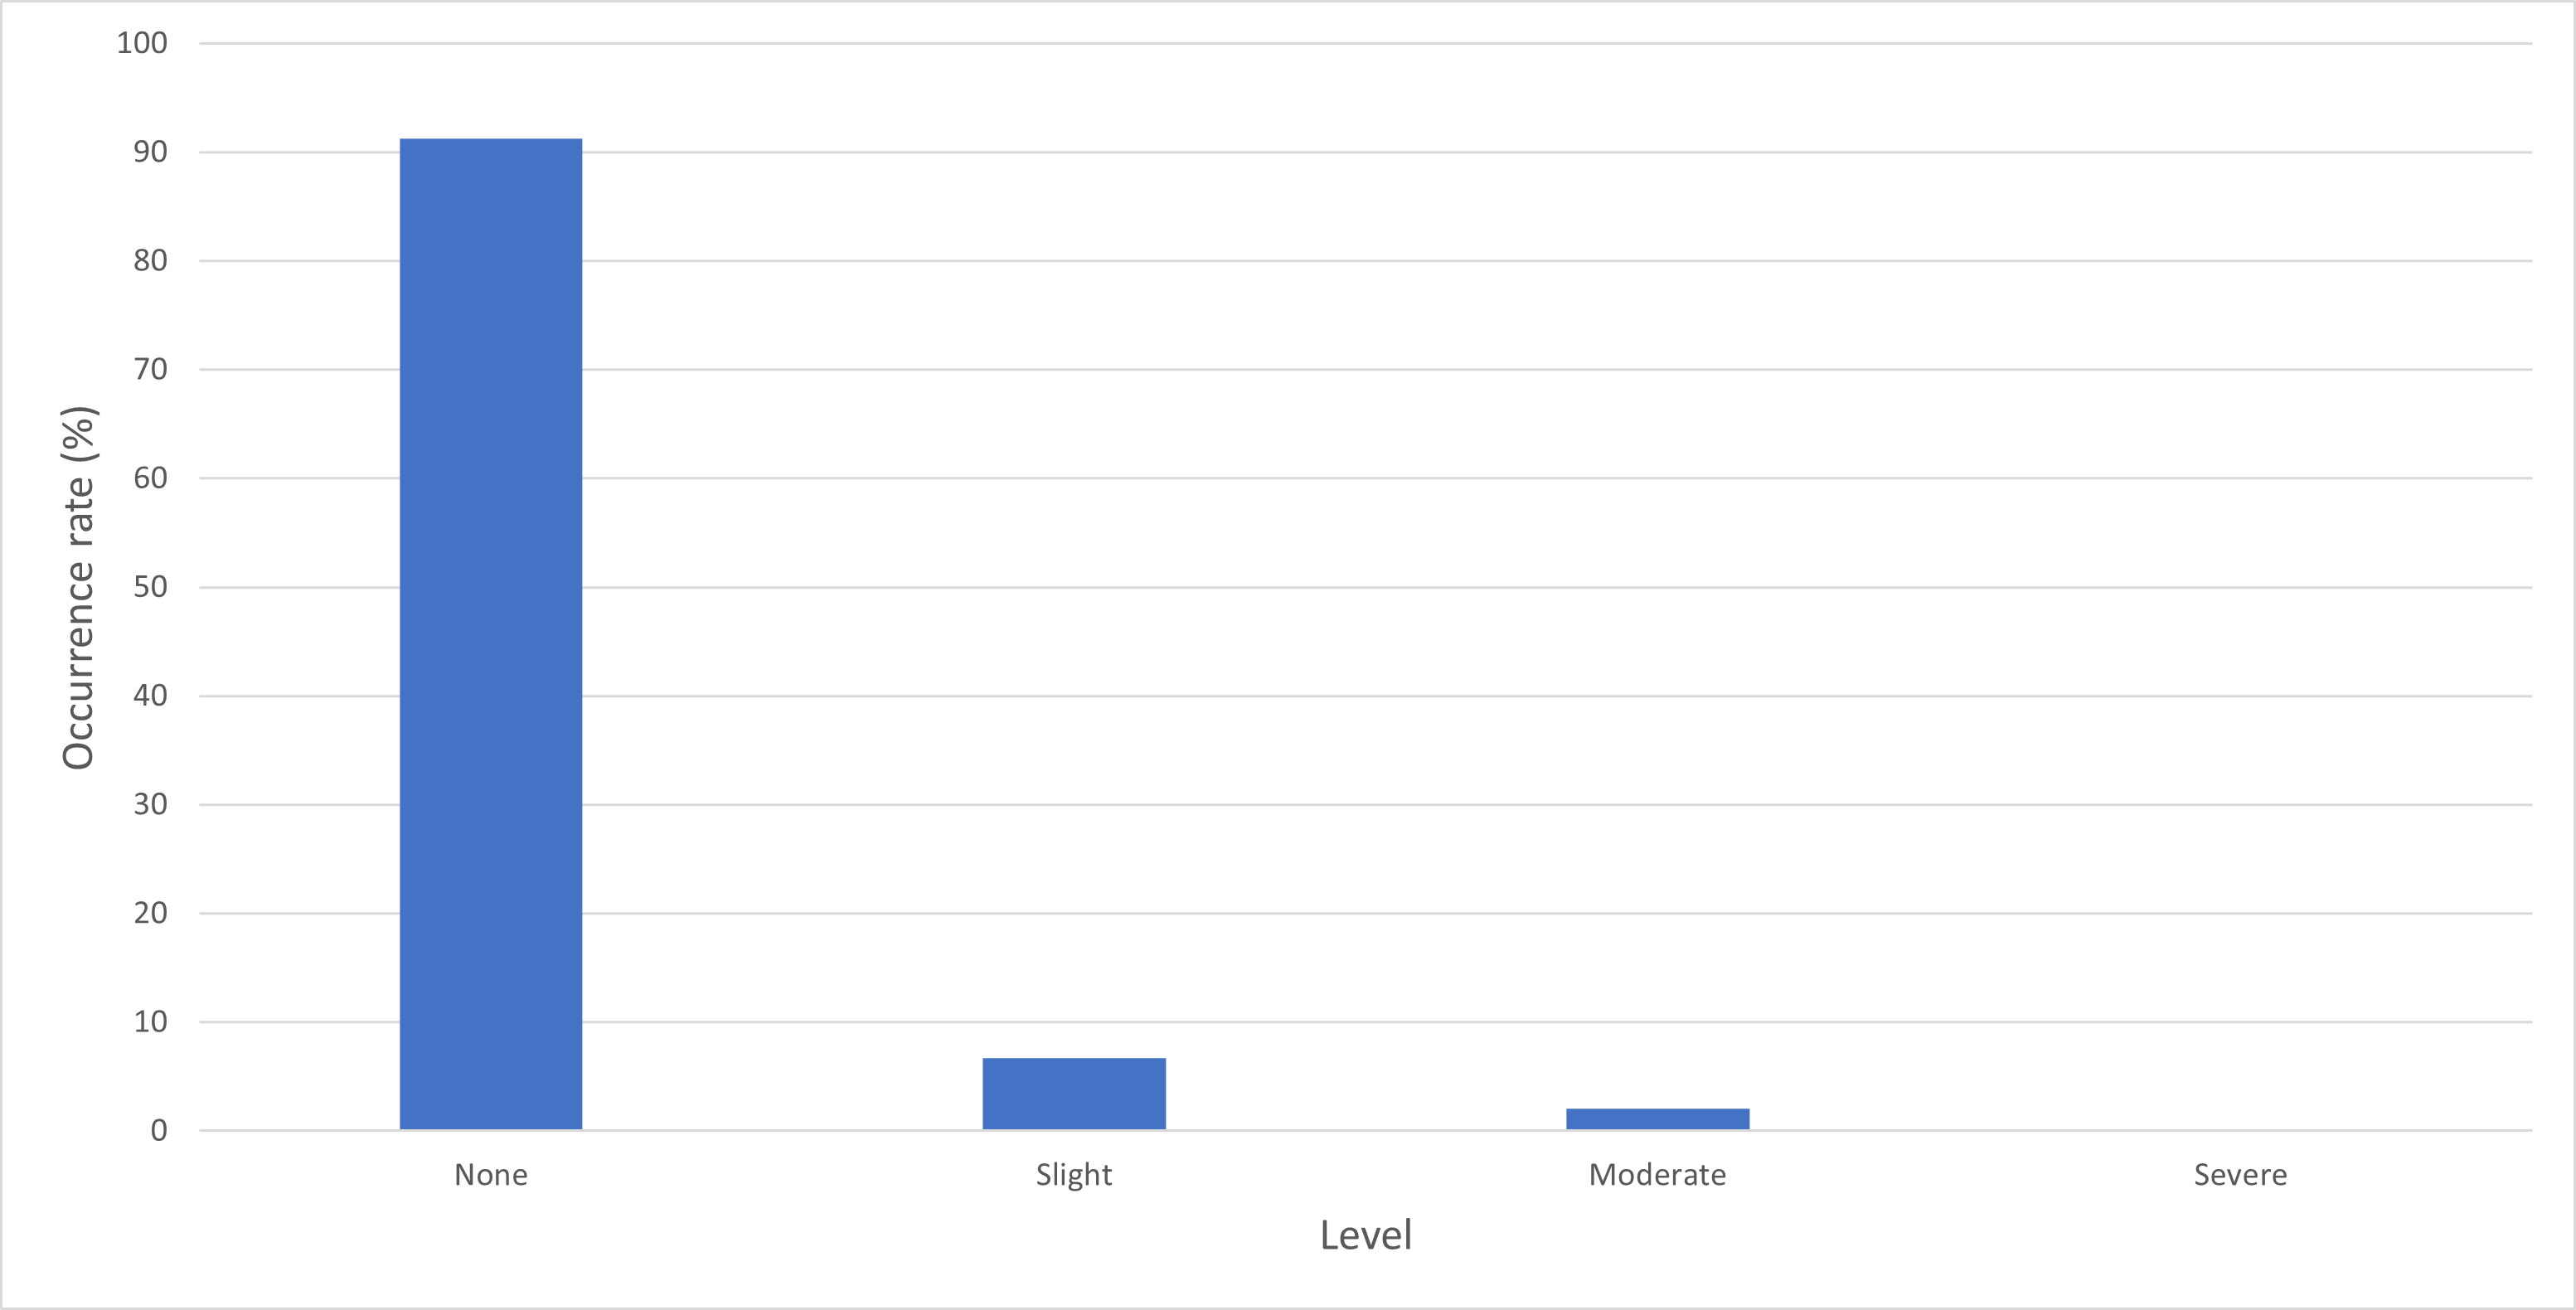
\includegraphics[width=0.9\textwidth]{Pictures/SSQ_Dec_Of_RotationEx.png}%imagine location
% 	\caption{SSQ results for the deceleration rotation task.}\label{fig:SSQ_Dec_Of_RotationEx}%use name for ref.
	
% \end{figure}
% \begin{figure}[H]\centering
% 	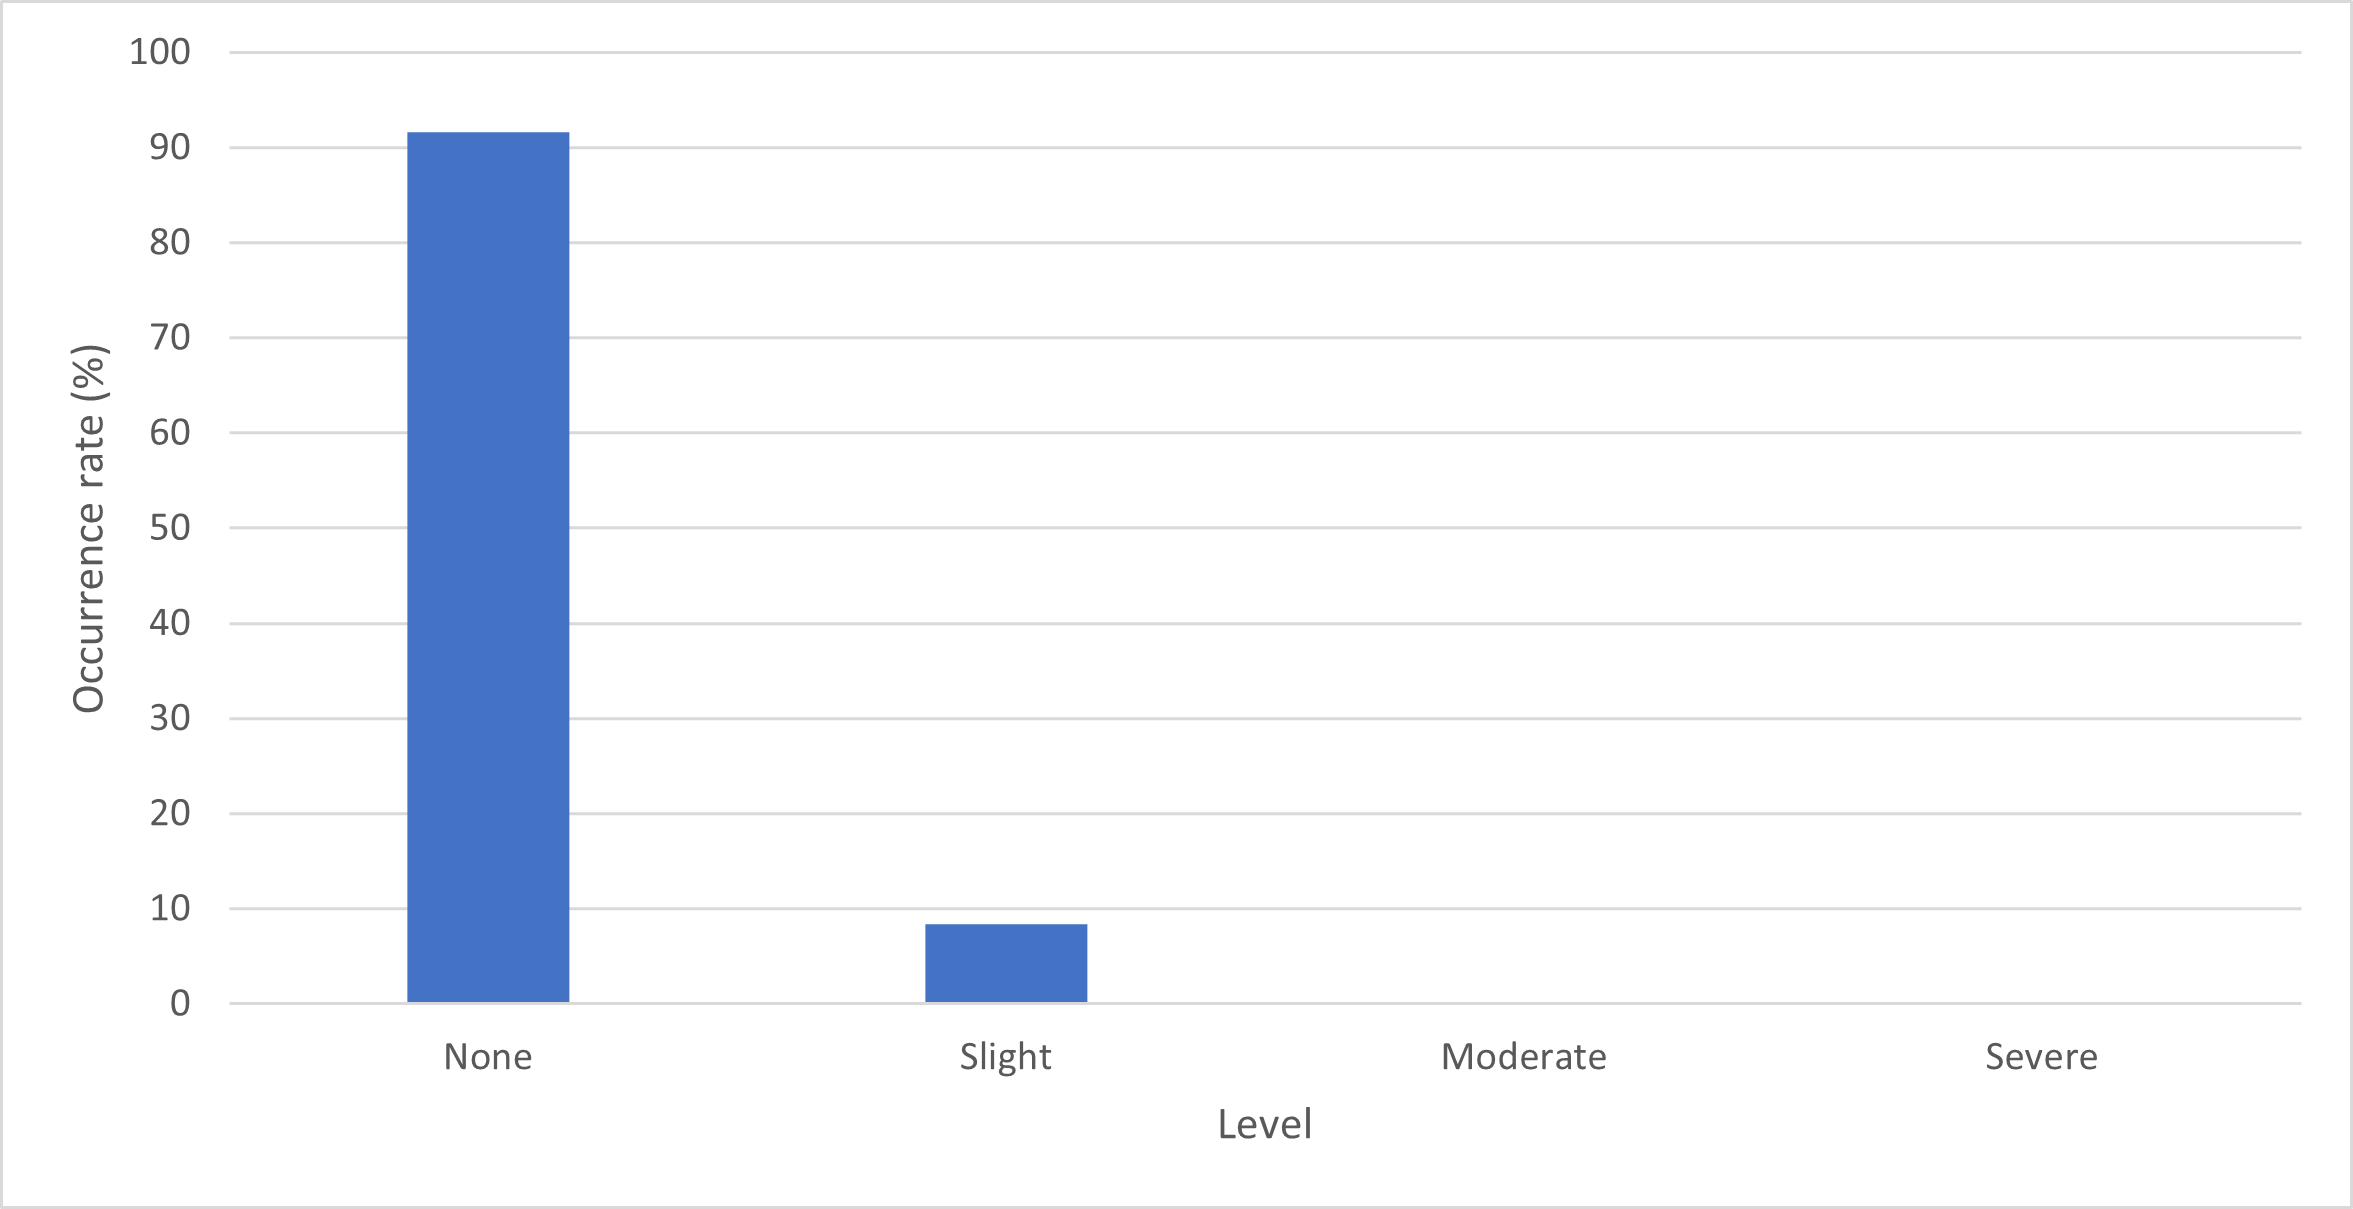
\includegraphics[width=0.9\textwidth]{Pictures/SSQ_Acc_Of_RotationEx.png}%imagine location
% 	\caption{SSQ results for the acceleration rotation task.}\label{fig:SSQ_Acc_Of_RotationEx}%use name for ref.

% \end{figure}
% \begin{figure}[H]\centering
% 	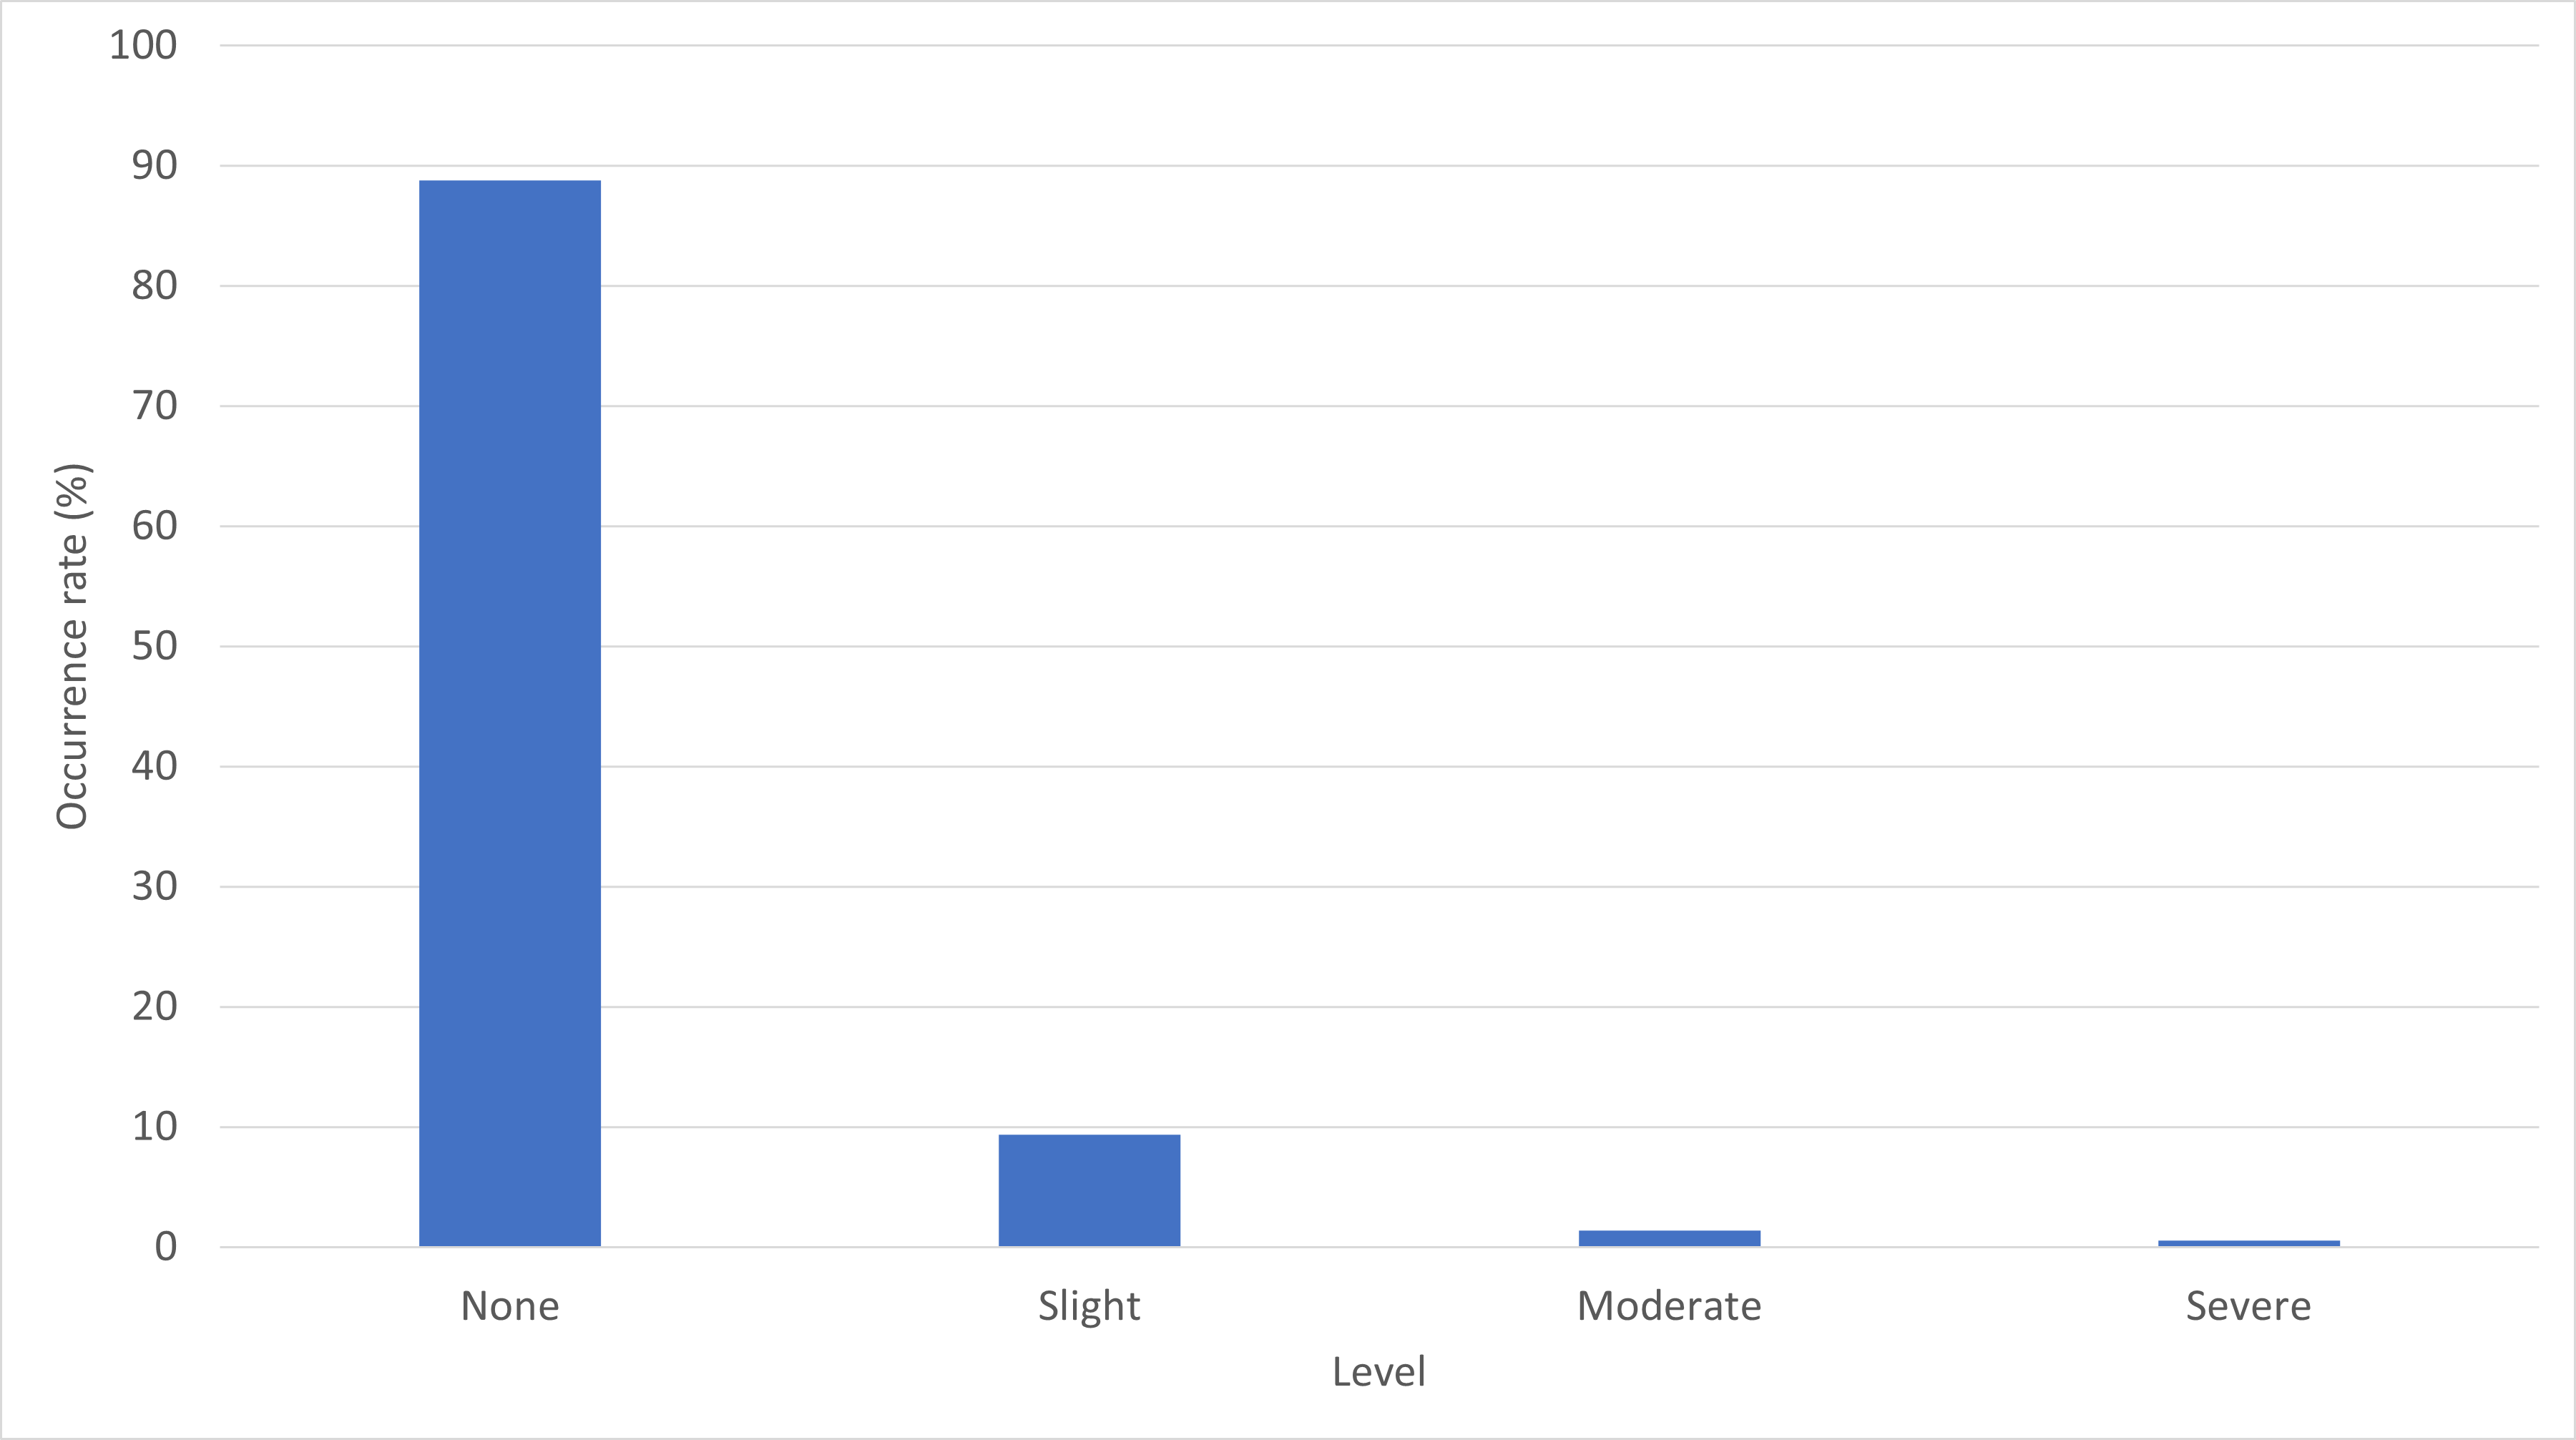
\includegraphics[width=0.9\textwidth]{Pictures/SSQ_ConstantOfCurvatureEx.png}%imagine location
% 	\caption{SSQ results for the constant speed task.}\label{fig:SSQ_ConstantOfCurvatureEx}%use name for ref.
	
% \end{figure}
% \begin{figure}[H]\centering
% 	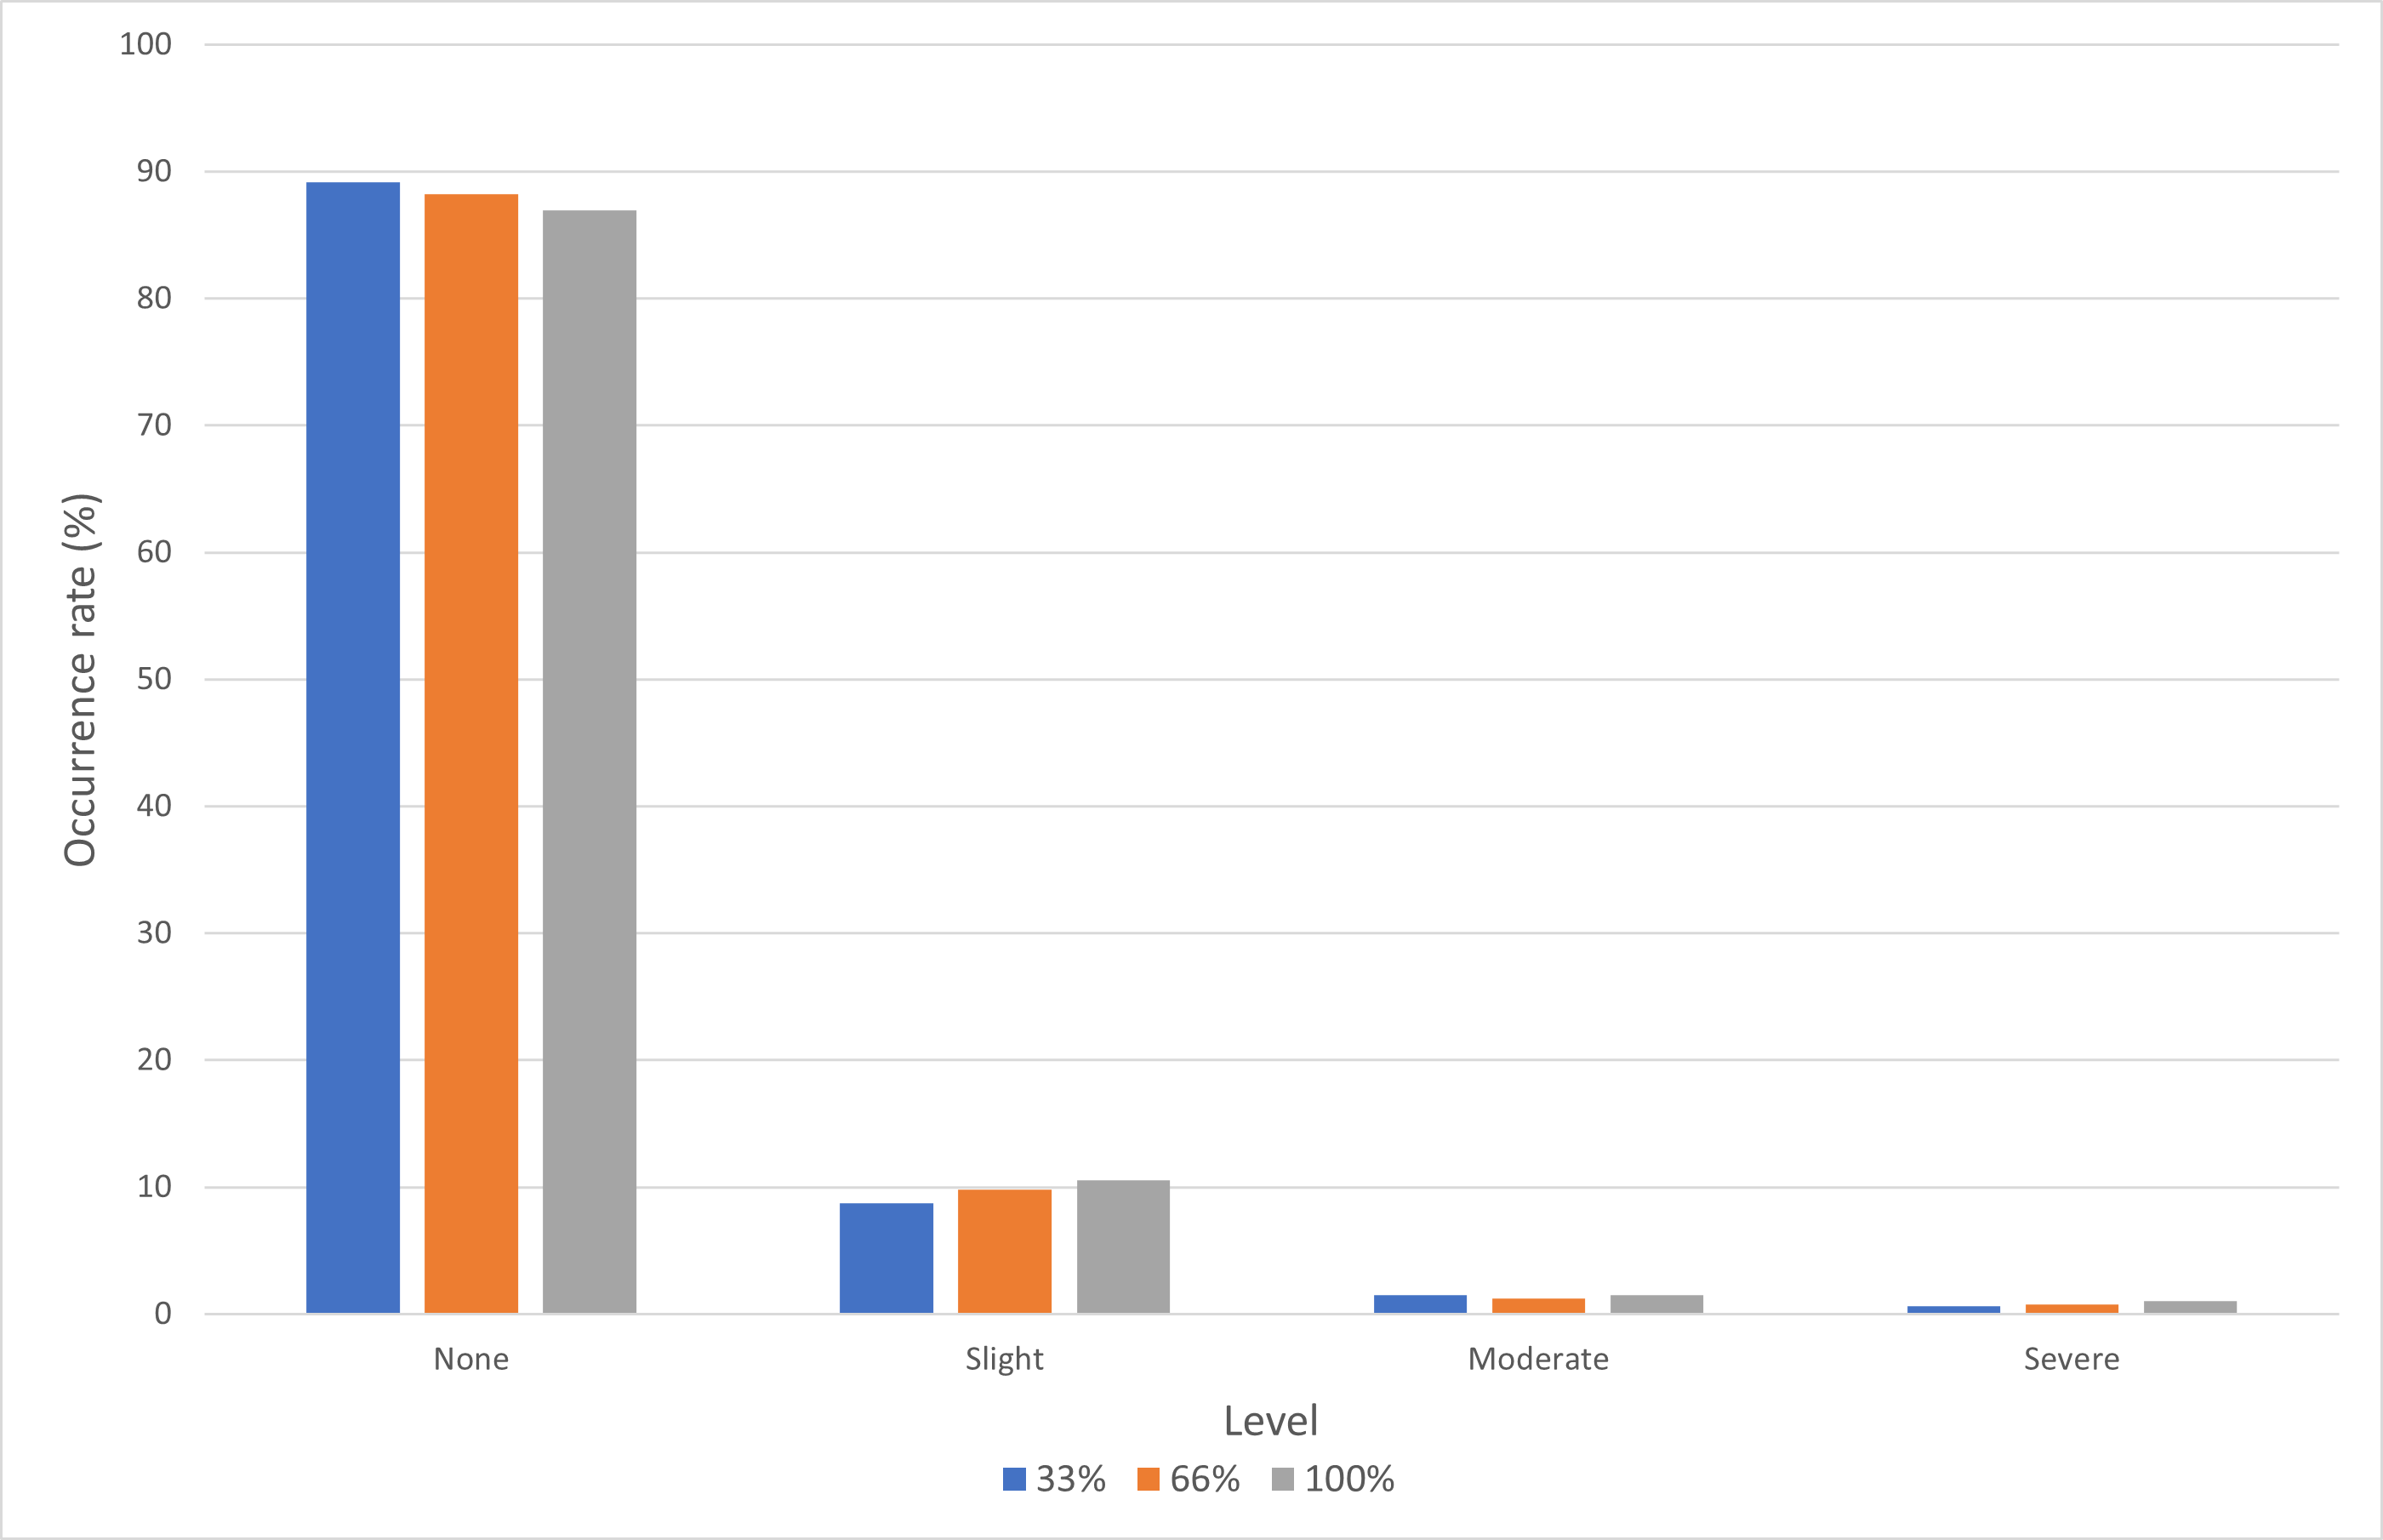
\includegraphics[width=0.9\textwidth]{Pictures/SSQ_AccOfCurvatureEx.png}%imagine location
% 	\caption{SSQ results for the acceleration task.}\label{fig:SSQ_AccOfCurvatureEx}%use name for ref.
	
% \end{figure}
% \section{Deployment in the real scenario}
% From the simulation result, collisions can be avoided efficiently by the proposed method. However, when the proposed method is applied to the real scenario, there should be room for discussion. The simulation of the proposed method has a restricted condition that is the speed of walking 0.5m/s. If it is more or less than 0.5 m/s, the collision avoidance would be possible to fail and the collision possibility would be high. The further experiment on the relation between the speed of walking, the speed of rotation, and curvature distance, are needed. 
% \section{Shapes of physical spaces}
% The proposed method was evaluated by simulation where the physical space was a rectangular room. Three sizes of physical spaces were taken into consideration: Large, Medium and Small. In the real scenario, there must be tables, bookshelves, sofas, etc. in a room, leading to a complicated walking space. It has an effect on the collision possibility. A further experiment on the relation between practical layouts of a room and performance of collision avoidance is needed. 
% \section{Effect of simulation frame rate on collision prediction}
% The simulation ran on the Unity engine in the experiment. In Unity, to advance the simulation each step, Update() function is called to change properties of objects before they are rendered at each frame. The interval between Update() calls varies depending on an amount of rendering loads. If the interval slowed down, the collision prediction would not work properly. Because each agent walks at the speed of 0.5m/s, the distance he/she travels between frames is 0.83cm when the frame rate is 60 frames per second or fps. Fig.~\ref{fig:framerate} shows the relation between frame rates and the number of agents. The lowest frame rate is 51.13629 and the distance each agent travels between frames is 0.978cm in that case. This frame rate is expected not to affect the collision prediction.
% %For testing the first experiment, we had a subject (5 people) and gave them to wear and try to notice the rotation in the virtual environment. We discussed and recorded the time for subjects to notice the rotation speed of (0.4deg/s, 0.8deg/s, 1.6deg/s, 3.2deg/s, 6.4deg/s and 12.8deg/s) when stop to constant speed and constant speed to stop rotation. In additional, we recorded the time for subjects to notice the deceleration and acceleration of (33\%, 66\% and 100\%) and the max rotation speeds are 0.4deg/s, 0.8deg/s, 1.6deg/s and 3.2deg/s. We knew the notice time of users, but we did not know about the rerated of a virtual environment and physical space distance in user moving situations. Also, while the user is walking the scene that we created in the program and we need them to rotate to make the curvature distance to avoid a collision with other users. We had to consider the average of half the width of a human shoulder (23cm) that affects the user's moving to avoid a collision with other users. So, we did another experiment that let the subject walk in a virtual environment and measured the distances in the constant speed task and acceleration task.
% %From the result of both experiments, we had enough of the actual situation's information to make the simulation for multiple users (2 to 15). Based on the previous experiments' data, we create the simulation that the colliding users will be rotated while walking to avoid the collision when the collision is detected. When more than two users collide, all of the colliding users will be rotated. From the discussion, we need to know the proposed method's efficiency, and then we find the other method for comparing. We found that Holm's method is often used to avoid collisions between users. Then, we create Holm's method simulation. As more than two users share a physical place, we concluded that the proposed method is better compared to Holm's way because when three or more users have predicted a collision at the same time, Holm's method can be enabled collision avoidance function for only even number of users. When the number of users becomes an odd number, Holm's method can not notice some users and fail to collision avoidance, but the proposed method can enable a collision avoidance function that can be predicted for a collision of multiple users. Also, the proposed method's count of collision is lower than Holm's method and the count of successful avoidance is higher than Holm's method.
% \begin{figure}[H]\centering
% 	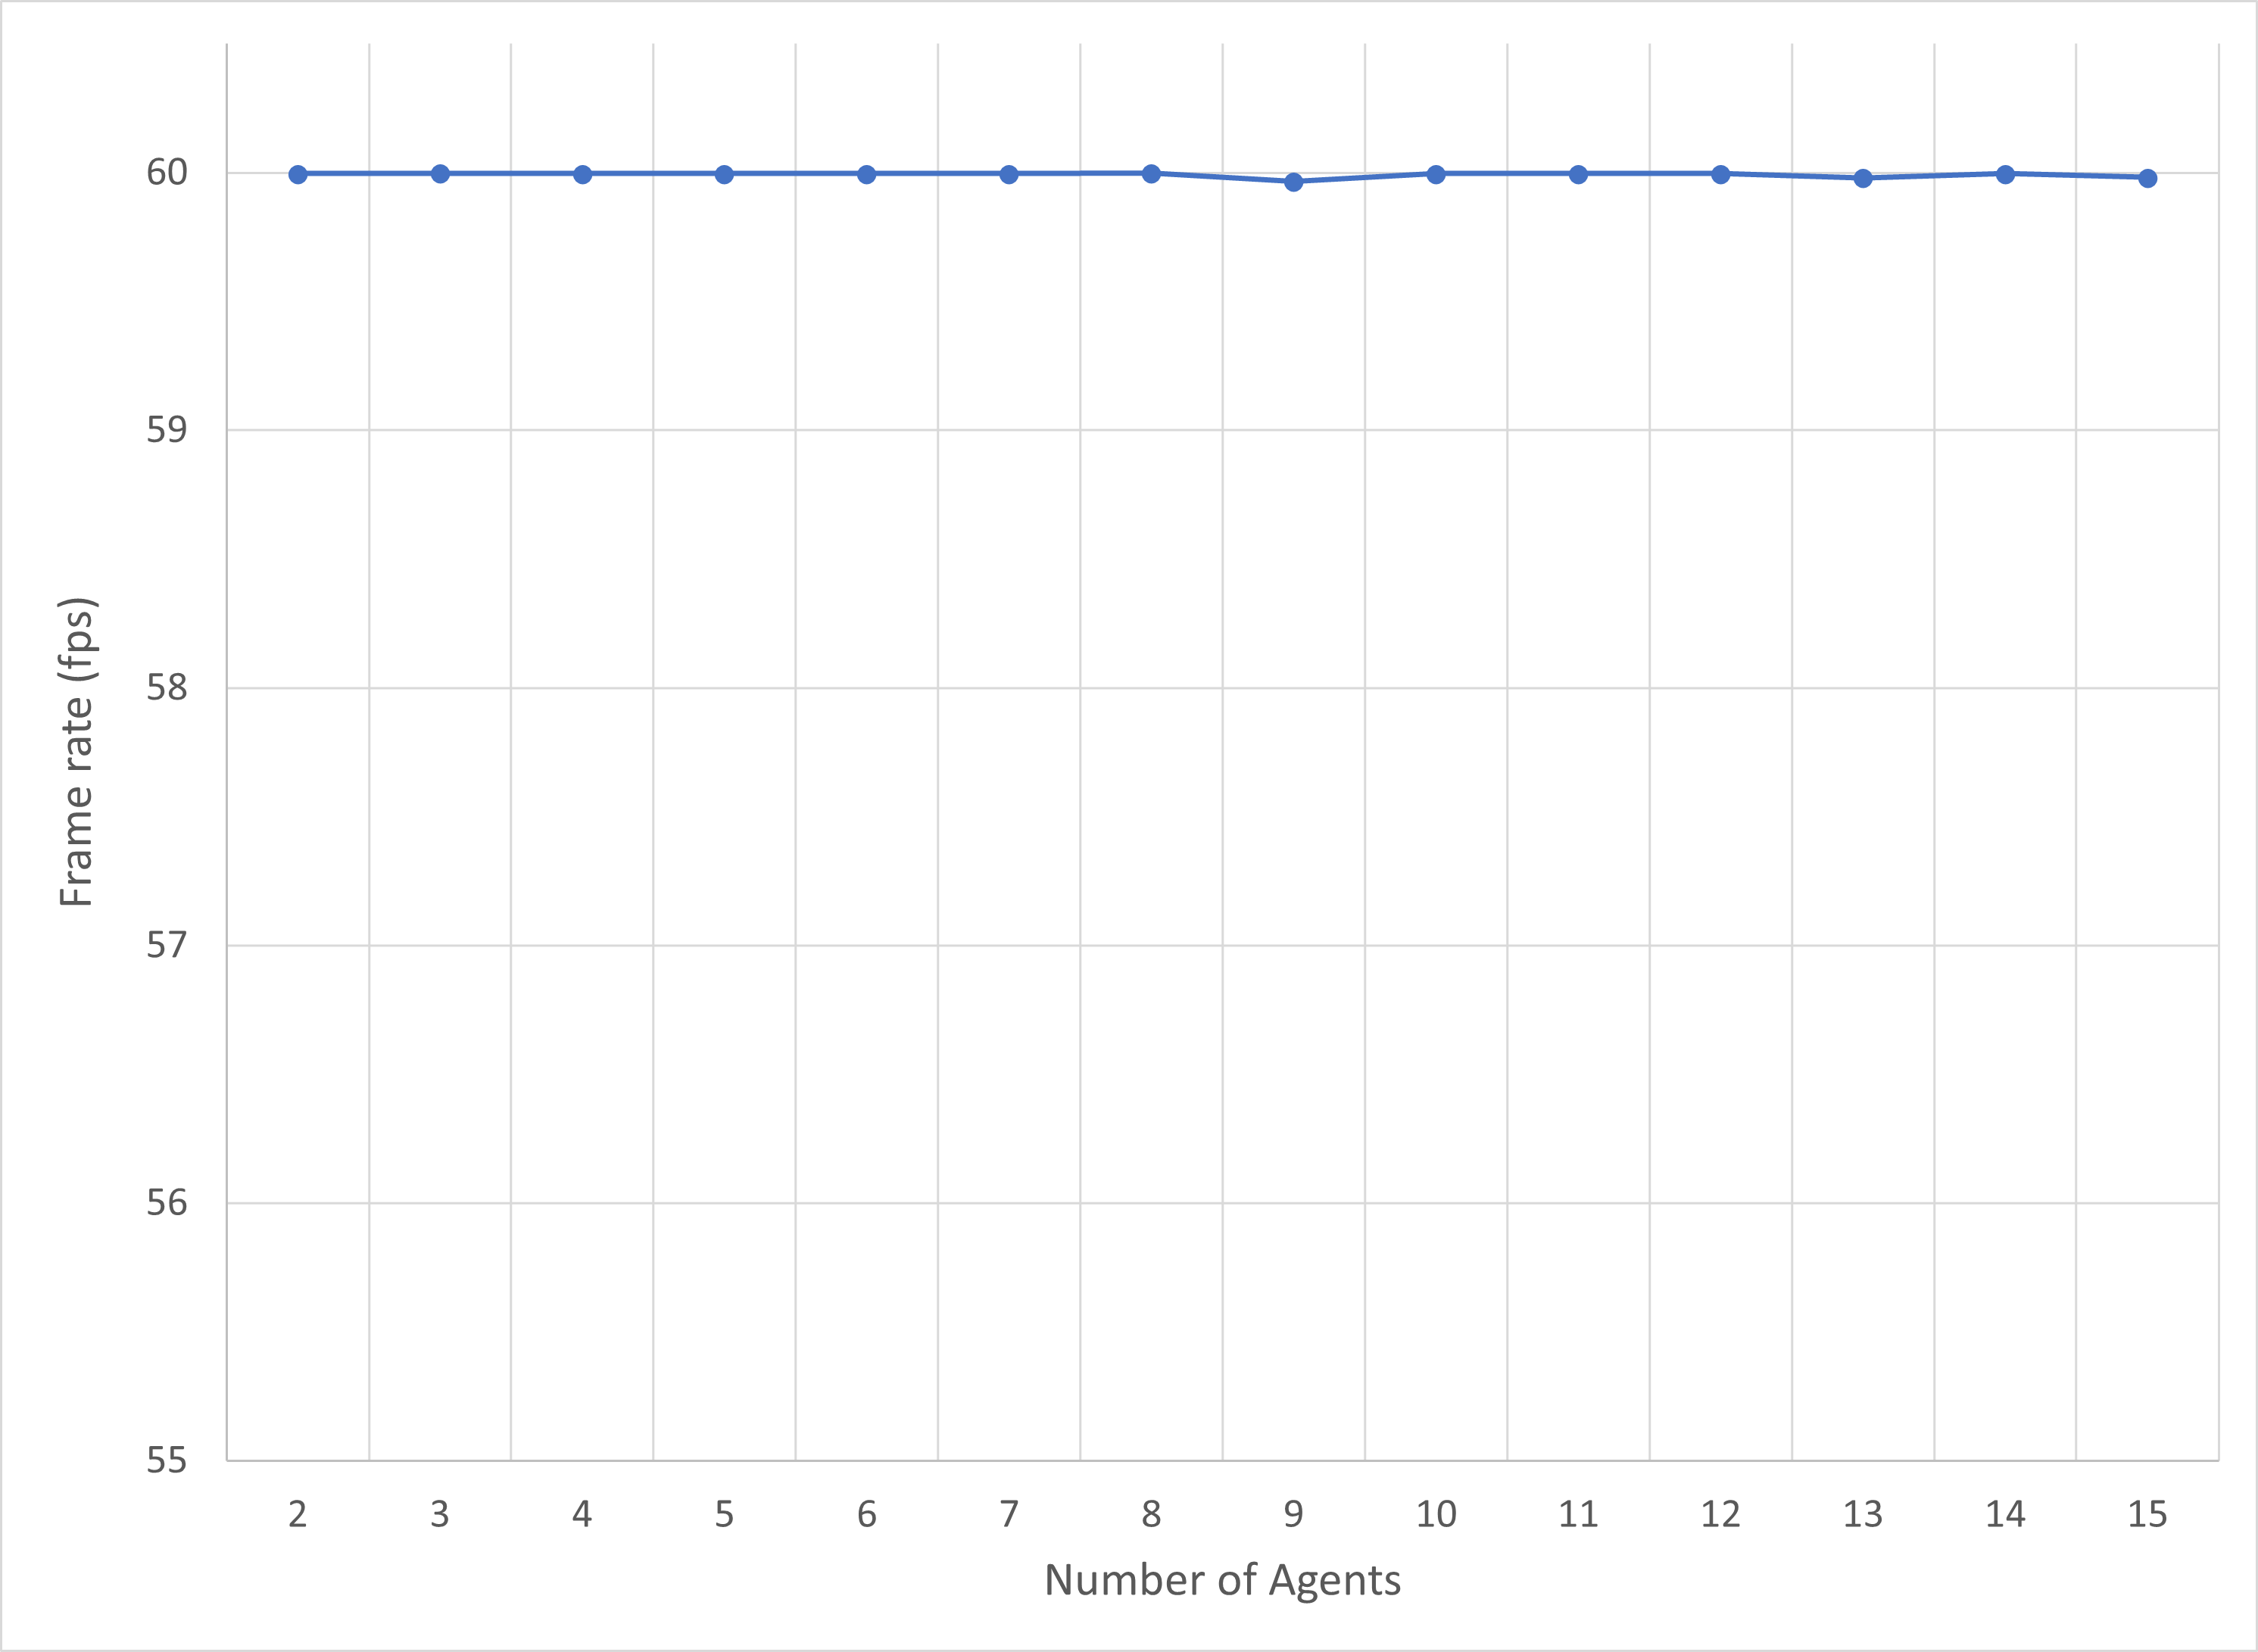
\includegraphics[width=1.0\textwidth]{Pictures/framerate.png}%imagine location
% 	\caption{Average of frame rate at each the number of agents.}\label{fig:framerate}%use name for ref.
	
% \end{figure}